\chapter{Охрана труда и окружающей среды}
\section{Анализ условий труда}
\subsection{Обеспечение условий труда в отделе разработки программного обеспечения}
Дипломная работа посвящена разработке системы мониторинга состояния ЛА на основе алгоритмов интеллектуального анализа данных. Разработка производится на персональном компьютере и предполагает длительное пребывание за ним инженера.

Применение персонального компьютера освобождает человека от непроизводительной работы, связанной с обработкой информации, изменяет характер его труда. Однако при этом увеличивается доля умственного и нервно-напряженного труда, возрастает психоэмоциональная нагрузка. При значительной трудовой нагрузке, нерациональной организации работы и неблагоприятных факторах производственной среды быстро снижается работоспособность операторов, уменьшается производительность труда и ухудшается качество работы, может развиться перенапряжение,~а в отдельных случаях возникнуть срыв трудовой деятельности~--- дистресс.

В данном разделе проводится анализ условий труда в отделе разработки информационных систем с целью обеспечения безопасности и удобства, требуемых для работы инженера.

\subsection{Характеристика помещения}
Помещение находится в здании Московского Авиационного Института и представляет собой кафедральную лабораторию со следующими размерами:
\begin{itemize}
	\item длина~6~м;
	\item ширина~4~м;
	\item высота~3.5~м.
\end{itemize}

Площадь: $6\times4 = 24$~м\textsuperscript{2}.

Объём: $6\times4\times3.5 = 84$~м\textsuperscript{3}.

Количество рабочих мест~---~4.

Количество одновременно находящихся в помещении сотрудников не превышает~4 человек.

План помещения приведён на рисунке~\ref{fig:labourprotection:room_plan}.

\begin{figure}[h]
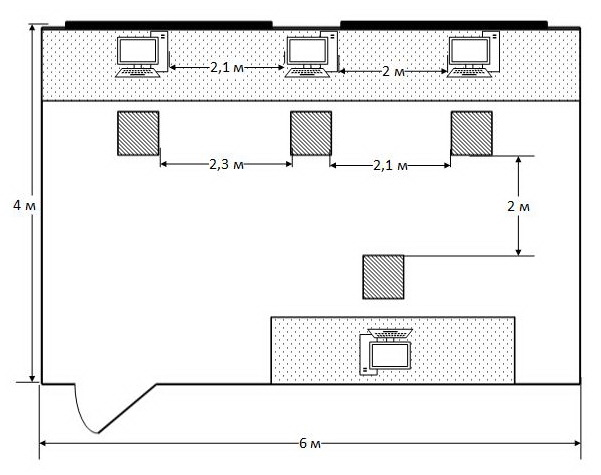
\includegraphics[width=0.6\textwidth, keepaspectratio]{room_plan}
\caption{План помещения}\label{fig:labourprotection:room_plan}
\end{figure}

Нормативные требования к площади и объёму рабочих мест определены в \cite{SanPin2_2_2}:
\begin{itemize}
	\item площадь на одно рабочее место с ВДТ или ПЭВМ для взрослых пользователей должна составлять не~менее~6~м\textsuperscript{2};
	\item объём~---~не~менее~20~м\textsuperscript{3}.
\end{itemize}

Фактические значения на каждого сотрудника:
\begin{itemize}
	\item площадь: $24/4 = 6$~м\textsuperscript{2};
	\item объём: $84/4 = 21$~м\textsuperscript{3}.
\end{itemize}

Данные значения показывают, что кафедральная лаборатория полностью соответствует установленным нормам.

В помещении имеются 2 оконных проёма высотой 1,6~м и шириной 2,3~м, которые выходят на юго-запад.

Искусственное освещение представляет собой 6~светильников, расположенных параллельно окнам в~2~ряда.

\subsection{Характеристика производственного процесса}
Разработка программного обеспечения производится на ПЭВМ с подключенными к ней периферийными устройствами.

\subsection{Характеристика используемого оборудования}
В процессе разработки используется следующее оборудование:
\begin{enumerate}
	\item{ПЭВМ:}
		\begin{enumerate}
			\item{процессор Intel Core i5 3,60 ГГц;}
			\item{оперативная память 8 Гб;}
			\item{жёсткий диск 1 Tб;}
			\item{напряжение питания 220 В.}
		\end{enumerate}
	\item{ЖК монитор с диагональю 23 дюйма (58,42) ASUS VX239H:}
		\begin{enumerate}
			\item{частота 75 Гц;}
			\item{яркость 250 кд/м\textsuperscript{2};}
			\item{динамическая контрастность 8 000 000 : 1;}
			\item{напряжение питания 220 В.}
		\end{enumerate}
	\item{Клавиатура Logitech K330;}
	\item{Мышь A7Tech X;}
	\item{Принтер HP LaserJet 1005M:}
		\begin{enumerate}
			\item{напряжение питания 220 В.}
		\end{enumerate}
\end{enumerate}

\subsection{Санитарно-гигиенические факторы}

\subsubsection{Микроклимат помещения}
Микроклимат в рабочем помещении должен соответствовать \cite{GOST12_1_005}.

Согласно \cite{GOST12_1_005}, работа разработчика ПО относится к категории «Легкая~–~Iа», т.к. лёгкие физические работы~--- работы с расходом энергии не более 150 ккал (174 Вт), а категория Iа подразумевает энергозатраты до 120~ккал/ч~(139 Вт).

Рабочее место разработчика ПО является постоянным, т.к. он находится на нём большую часть рабочего времени (более~50\%).

Нормативные и фактические значения для категории работ «Легкая~–~Iа», лёгкие физические работы~--–~работы с расходом энергии не более 150~ккал (174~Вт). Категория Iа подразумевает энергозатраты до 120~ккал/ч (139~Вт).

Рабочее место разработчика модели является постоянным, т.к. он находится на нём большую часть рабочего времени (более 50\%).

Нормативные и фактические значения для категории работ «Легкая – Iа» и постоянного рабочего места приведены в таблице~\ref{tab:labourprotection:microclimat}.

\begin{table}[h]
\caption{Значения характеристик микроклимата помещения}
\label{tab:labourprotection:microclimat}
\nohyphenation

\begin{tabular}{|C{84pt}|C{178.25pt}|C{101.1pt}|C{110pt}|}
\hline
 & Температура, \textdegree C & Относительная влажность, \% & Скорость движения, м/с \\
\hline
Допустимые значения & 22--24~–-- Холодный период \linebreak 23--25~--– Теплый период & 40--60 & 0.1 \\
\hline
Фактические значения & 22--24~–-- Холодный период \linebreak 25--30~--– Теплый период & 45--55 & <0.1 \\
\hline
\end{tabular}
\end{table}

Фактические значения параметров микроклимата данного помещения удовлетворяют допустимым значениям для холодного периода года. Во время теплого периода в помещении может преобладать повышенная температура из-за отсутствия кондиционера, который бы мог её регулировать.

\subsubsection{Производственное освещение}
Освещённость регламентируется~\cite{SNiP23_05_95}.

Наименьший размер объекта различения в работе инженера составляет 0.3 мм. Объектом является символ, выводимый на экран монитора (наименьшим символом является точка). Зрительная работа относится к III разряду --- высокая точность (наименьший размер объекта различения от 0.3 до 0.5~мм).

Контраст объекта с фоном средний, фон светлый, что соответствует подразряду~б разряда III.

Требования к освещению помещений промышленных предприятий для подразряда~б разряда III:
\begin{itemize}
	\item При системе комбинированного освещения освещенность равна: всего --- 1000 лк, в т.ч. от общего --- 200 лк;
	\item При системе общего освещения освещённость равна 300 лк.
\end{itemize}

Система освещения в комнате общая, состоящая из 6 потолочных светильников ЛПО 46, в каждом из которых установлены 4 люминесцентные лампы ЛТБ мощностью 20 Вт и световым потоком 1100 лм. Светильники расположены в два ряда параллельно окнам. Фактическая освещенность составляет 275 лк, что полностью удовлетворяет нормативным значениям~\cite{SNiP23_05_95}.

\subsubsection{Шум}
Источники шума в данном помещении: охлаждающие системы ПЭВМ (охлаждение процессоров).

Уровни шума на рабочих местах инженера ПЭВМ должны соответствовать~\cite{GOST12_1_003}.

Допустимые значения уровня шума при проектировании и программировании на рабочих местах в помещениях проектно-конструкторских бюро; расчётчиков, программистов вычислительных машин, в лабораториях для теоретических работ и обработки данных: не более  50 дБА.

Фактические значения уровня шума: не более 45 дБА, что подтверждается расчётами в разделе~\ref{sec:labourprotection:calc}.

Согласно~\cite{GOST12_1_003}, значения уровня шума на рабочем месте удовлетворяют установленным требованиям.

\subsubsection{Электромагнитное излучение}
Во время работы ПЭВМ возникают электромагнитные поля, которые оказывают негативное влияние на организм человека.

Источниками электромагнитных полей на рабочем месте инженера являются системные блоки. Современные корпуса системных блоков ПЭВМ позволяют значительно ослабить излучения его элементов. Благодаря существующим достаточно строгим стандартам дозы рентгеновского излучения от современных мониторов и системных блоков не опасны для пользователей.

Документом, регламентирующим уровень электромагнитного излучения для ПЭВМ, является~\cite{SanPin2_2_2}.

Согласно ему, напряжённости электрических и магнитных полей, энергетической нагрузки в течение рабочего дня не должны превышать значений, указанных в таблице~\ref{tab:labourprotection:emradiation}.

\begin{table}[h]
\caption{Предельные значения электромагнитного излучения.}
\label{tab:labourprotection:emradiation}
\nohyphenation

\begin{tabular}{|C{213.35pt}|C{87.35pt}|C{84.4pt}|C{83.4pt}|}
\hline
\multirow{2}{\hsize}{\centering{Параметр}} & \multicolumn{3}{C{255.15pt}|}{Предельные значения в диапазонах частот, МГц} \\
\cline{2-4}
 & от 0.06 до 3 & св. 3 до 30 & св. 30 до 300 \\
\hline
$\text{Е}_\text{ПД}, \text{В/м}$ & 500 & 300 & 80 \\
\hline
$\text{Н}_\text{ПД}, \text{А/м}$ & 50 & --- & --- \\
\hline
$\text{ЭН}_{\text{Е}_\text{ПД}}, \text{(В/м)}^2 \cdot \text{ч}$ & 20000 & 7000 & 800 \\
\hline
$\text{ЭН}_{\text{Н}_\text{ПД}}, \text{(А/м)}^2 \cdot \text{ч}$ & 200 & --- & --- \\
\hline
\end{tabular}
\end{table}

Монитор ASUS VX239H соответствует стандарту~\cite{TCO03}, который устанавливает следующие предельные значения электромагнитного излучения:
\begin{itemize}
	\item напряжённость электрического поля: в диапазоне 5Гц--2кГц не более 10~В/м, в диапазоне 2кГц--400кГц не более 1.0~В/м;
	\item напряжённость магнитного поля: в диапазоне 5Гц--2кГц не более 200~нТл, в диапазоне 2кГц--400кГц не более 25~нТл.
\end{itemize}

Данные характеристики полностью соответствуют требованиям~\cite{SanPin2_2_2}.

\subsection{Электроопасность}
В данном помещении используется оборудование, питающееся от сети переменного тока напряжением 220~В, частотой 50~Гц. 

Согласно~\cite{PUE7}, помещение отдела разработки ИС относится к классу помещений без повышенной опасности поражения электрическим током: это сухое помещение с непроводящими полами, с нормальной температурой воздуха и влажностью, в нем отсутствует токопроводящая пыль.

Электрооборудование в помещении представлено мониторами и системными блоками ПЭВМ. Источником электрического поражения может быть металлический корпус системного блока при пробое изоляции, т.к. имеется напряжение 220~В, а в~\cite{GOST12_1_038} допустимое напряжение и ток для аварийных режимов при времени воздействия более 1~секунды составляют 20~В и 6~мА.

\subsection{Пожароопасность}
В данном помещении имеются твердые горючие и  трудногорючие веще-ства и материалы (книги, документы, деревянная мебель, оргтехника и т.д.), которые при взаимодействии с огнем будут гореть без взрыва. Также источником возгорания может быть электрическая проводка.

Согласно~\cite{GOST12_1_004}, данное помещение относится к классу Б и является пожароопасным.

\subsection{Эргономические факторы}
Требования к организации рабочих мест пользователей ПЭВМ изложены в~\cite{SanPin2_2_2}. 

Согласно~\cite{SanPin2_2_2}, расстояние между рабочими столами с мониторами (в направлении тыла поверхности одного монитора и экрана другого монитора) должно быть не менее 2~м, а расстояние между боковыми поверхностями мониторов не менее 1.2~м.

Фактические значения (см. рисунок~\ref{fig:labourprotection:room_plan}):
\begin{itemize}
	\item расстояние между рабочими столами 2.1--2.5~м;
	\item расстояние между боковыми поверхностями мониторов 2.1-2.3~м.
\end{itemize}

Таким образом, размещение рабочих столов полностью соответствуют требованиям~\cite{SanPin2_2_2}.

В помещении используется специальный стол~--– рабочая поверхность, изготовленная на заказ по выбранным заказчиком параметрам. Ее характеристики и нормативные значения указаны в таблице~\ref{tab:labourprotection:desktop}.

\begin{table}[h]
\caption{Характеристики используемого рабочего стола}
\label{tab:labourprotection:desktop}
\nohyphenation

\begin{tabular}{|C{225.9pt}|C{125.05pt}|C{114.85pt}|}
\hline
Наименование параметра & Нормативное значение~\cite{SanPin2_2_2}, мм & Фактическое значение, мм \\
\hline
Ширина рабочей поверхности & не менее 500  & 1200--2000 \\
\hline
Глубина рабочей поверхности & не менее 800 & 800 \\
\hline
Высота рабочей поверхности & не менее 725 & 800 \\
\hline
Пространство для ног высотой & не менее 600 & 600 \\
\hline
Глубина на уровне колен & не менее 450 & 450 \\
\hline
Глубина на уровне вытянутых ног & не менее 650 & 650 \\
\hline
\end{tabular}
\end{table}

Параметры стола полностью соответствуют требованиям~\cite{SanPin2_2_2}.

В помещении используется офисное кресло БЮРОКРАТ Ch-G318AXN. Его характеристики и нормативные размеры указаны в таблице~\ref{tab:labourprotection:chair}.

%\begin{table}[h]
\begin{longtable}{|C{197.55pt}|C{153.4pt}|C{114.85pt}|}
\caption{Характеристики используемого офисного кресла}
\label{tab:labourprotection:chair}
\\\hline
Наименование параметра & Нормативное значение~\cite{SanPin2_2_2} & Фактическое значение \\
\endhead
\hline
Ширина и глубина поверхности сиденья & не менее 400 мм & 420 мм \\
\hline
Регулировка высоты поверхности сиденья  & 400--550 мм & 440--570 мм \\
\hline
Регулировка углов наклона сиденья & вперед до 15\textdegree и назад до 5\textdegree & вперед до 15\textdegree и назад до 5\textdegree \\
\hline
Высота опорной поверхности спинки & 300 ± 20 мм & 310 мм \\
\hline
Ширина опорной поверхности спинки & не менее 380 мм & 380 мм \\
\hline
Радиус кривизны горизонтальной плоскости опорной поверхности спинки & 400 мм & 400 мм \\
\hline
Угол наклона спинки в вертикальной плоскости & ± 30\textdegree & ± 30\textdegree \\
\hline
Регулировка расстояния спинки от переднего края сиденья & 260--400 мм & 260--450 мм \\
\hline
Стационарные или съёмные подлокотники & длина не менее 250 мм \linebreak ширина 50--70 мм & длина 250 мм \linebreak ширина 60 мм \\
\hline
Регулировка подлокотников по высоте над сиденьем & 230 ± 30 мм & Нет \\
\hline
Регулировка внутреннего расстояния между подлокотниками & 350--500 мм & 420--500 мм \\
\hline
\end{longtable}
%\end{table}

Параметры стула частично не соответствуют требованиям \cite{SanPin2_2_2}: в данном рабочем кресле отсутствует регулировка подлокотников по высоте над сидением.

\subsection{Психофизиологические факторы}
Факторами, оказывающими влияние на внимательность инженера и его производительность труда, в условиях его рабочего места являются:
\begin{itemize}
	\item визуальные характеристики монитора (его яркость, контрастность, разрешение, частота обновления); 
	\item напряженность работы; 
	\item количество обрабатываемой информации –-- плотность воспринимаемых сигналов.
\end{itemize}

Используется ЖК монитор ASUS VX239H. Его фактические характеристики и нормативные значения~\cite{SanPin2_2_2} приведены в таблице~\ref{tab:labourprotection:display}.

\begin{table}[h]
\caption{Характеристики используемого ЖК монитора}
\label{tab:labourprotection:display}
\nohyphenation

\begin{tabular}{|C{178.9pt}|C{152.25pt}|C{158.9pt}|}
\hline
Наименование фактора & Действительное значение & Нормативное значение~\cite{SanPin2_2_2} \\
\hline
Размер экрана по диагонали & 58,42 см & не менее 31 см \\
\hline
Удалённость экрана & 60 см & не менее 50 см \\
\hline
Частота обновления изображения & 75 Гц & не менее 75 Гц \\
\hline
Контрастность & 8 000 000:1 & не менее 3:1 \\
\hline
Яркость знака & 250 кд/м2 & не менее 35 кд/м2 \\
\hline
\end{tabular}
\end{table}

Характеристики монитора полностью соответствуют требованиям~\cite{SanPin2_2_2}.

Напряженность работы на основании данных таблицы классов условий труда по показателям напряженности трудового процесса \cite{R2_2_2006} представлена в таблице~\ref{tab:labourprotection:workintensity}.

\begin{longtable}{|C{165pt}|C{165pt}|C{160pt}|}
\caption{Напряженность работы}
\label{tab:labourprotection:workintensity}
\\\hline
Критерий & Характеристика & Напряженность трудового процесса \\
\endfirsthead
\LTcontcaption{tab:labourprotection:workintensity}
\\\hline
Критерий & Характеристика & Напряженность трудового процесса \\
\endhead

\hline
Содержание работы & Решение сложных задач по известным алгоритмам (работа по серии инструкций) & Напряженный труд 1 степени \\
\hline
Восприятие сигналов (информации и их оценка) & Восприятие сигналов с последующей комплексной оценкой взаимосвязанных параметров & Напряженный труд 2 степени \\
\hline
Степень сложности задания & Обработка, проверка и контроль за выполнением задания & Напряженность труда средней степени \\
\hline
Характер выполняемой работы & График с возможной корректировкой & То же \\
\hline
Длительность сосредоточенного наблюдения (в \% от времени смены) & 26--50\% & --//-- \\
\hline
Плотность сигнала за 1 час работы & 176--300 & Напряженный труд 1 степени \\
\hline
Число объектов одновременного наблюдения & 6--10 & Напряженность труда средней степени \\
\hline
Размер объекта различения, мм, при длительном сосредоточенном наблюдении (\% времени смены) & 3--10 мм до 50\% времени & То же \\
\hline
Степень ответственности & Ответственность за качество конечного результата & Напряженный труд 2 степени \\
\hline
Значимость ошибки & Влечет за собой дополнительные усилия в работе со стороны работника & Напряженность труда лёгкой степени \\
\hline
Продолжительность рабочего дня & 8--9 часов & Напряженность труда средней степени \\
\hline
\end{longtable}

Среднее значение по данным критериям соответствует средней степени напряженности труда.

\section{Мероприятия по обеспечению условий труда}
Микроклимат в помещении в холодное время года обеспечивается с помощью системы центрального отопления. В летний же период времени в помещении не происходит регулирования температуры и влажности из-за отсутствия кондиционера. Рекомендуется установить, например, потолочный кондиционер Panasonic CS-A18BTP/CU-A18BBP5 с циркуляцией воздуха 840~м\textsuperscript{3}/час.

Мероприятия по обеспечению требуемых условий по освещенности можно отнести к выбору ламп в источниках света. Часть цвет предметов освещенных люминесцентными лампами может быть несколько искажён и быть неприятен человеку. Это, в свою очередь, вызывает усталость и напряженность глаз. Для предотвращения этого целесообразно использовать лампы с «трехполосным» и «пятиполосным» люминофором~--- веществом, способным преобразовывать поглощаемую им энергию в световое излучение. Это позволяет добиться более равномерного распределения излучения по видимому спектру, что приводит к более натуральному воспроизведению света. Данным параметрам соответствует лампа Philips Master~TL-D De~Luxe~36W/D65.

Уровень шума при использовании описанных ПЭВМ не превосходит норм, поэтому дополнительных мер для предотвращения излишнего шума не требуется. При закупке нового оборудования следует учитывать уровень шума от каждой новой единицы.

Обеспечение электробезопасности основано на применении устройств защитного отключения (УЗО). Данное устройство реагирует на ухудшение изоляции электропроводки: когда ток утечки повысится до предельной величины 30 мА, происходит отключение напряжения в течение 30 микросекунд. Целесообразно применять УЗО Legrand DX~06576.

Пожаробезопасность должна быть обеспечена при помощи обработки жидкостью от возгорания предметов мебели, инструктажа персонала на предмет мер предотвращения пожара или эвакуационных действий при пожаре, тщательной проверки оборудования на предмет повреждения проводов или оборудования.

\section{Расчетная часть}\label{sec:labourprotection:calc}
\subsection{Расчет уровня шума}
Цель расчета~–-- определить, соответствует ли фактический уровень шума в помещении нормативным значениям. Основными источниками шума в рассматриваемом помещении является аппаратура системных блоков ПЭВМ (кулер процессора).

Расчет производится в соответствии с~\cite{LabourProtOnCC}.

План помещения с указанием рабочих мест и рабочей точки показан на рисунке~\ref{fig:labourprotection:room_plan_wp}

\begin{figure}[h]
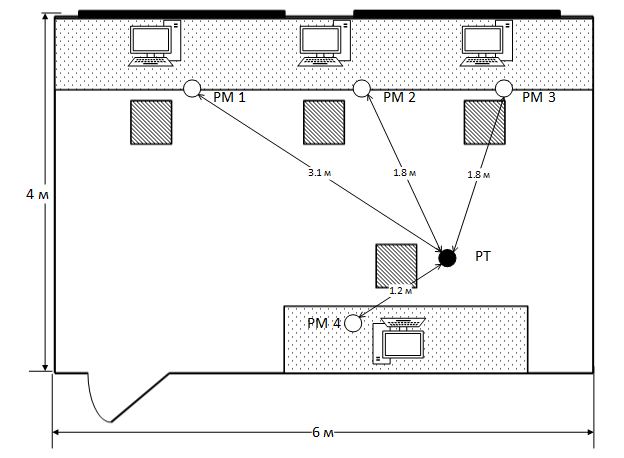
\includegraphics[width=0.67\textwidth, keepaspectratio]{room_plan_wp}
\caption{План помещения с указанием рабочих мест и рабочей точки}\label{fig:labourprotection:room_plan_wp}
\end{figure}

Будем считать, что оператор, находящийся в расчётной точке,  располагается в зоне действия прямого звука. Тогда фактические значения уровней звукового давления в октановых полосах частот на расстоянии $r$ от источника и суммарных значений от нескольких источников рассчитываются по формулам~\ref{eq:labourprotection:noise}~и~\ref{eq:labourprotection:noisesum}.

\begin{equation}\label{eq:labourprotection:noise}
L_i = L_{W_i} - 20 \cdot \log{r_i} - 11 \text{;}
\end{equation}
\begin{equation}\label{eq:labourprotection:noisesum}
L_{\sum} = 10 \cdot \log{\sum_{i=1}^{n} 10^{0.1 \cdot L_i}} \text{,}
\end{equation}
\begin{description}
	\item[где $L_{W_i}$] --- уровень звуковой мощности $i$-го источника.
\end{description}
\smallskip

Допустимые уровни звукового давления в расчётной точке представлены в соответствии с~\cite{SanPin2_2_2}.

Расстояния от рабочих мест до рабочей точки:

\smallskip
$r_1 = 1.8 \text{м}, r_2 = 1.8 \text{м}, r_3 = 3.1 \text{м}, r_4 = 1.2 \text{м}.$
\smallskip

Уровни звукового давления для источников шума 1-4 (РМ1-РМ4) для уровня звуковой мощности кулера $L = 38 \text{ дБ}$ и среднегеометрической частоты 500 Гц:

\smallskip
$\begin{aligned}
L_1 = 38 - 20 \cdot \log{1.8} - 11 = 31.9 \text{ дБ;}\\
L_2 = 38 - 20 \cdot \log{1.8} - 11 = 31.9 \text{ дБ;}\\
L_3 = 38 - 20 \cdot \log{3.1} - 11 = 27.2 \text{ дБ;}\\
L_4 = 38 - 20 \cdot \log{1.2} - 11 = 38.5 \text{ дБ.}\\
\end{aligned}$
\smallskip

В этом случае уровень звукового давления от 4 источников:

\smallskip
$L_{\sum} = 10 \cdot \log(10^{0.1 \cdot 31.9} + \log(10^{0.1 \cdot 31.9} + \log(10^{0.1 \cdot 27.2} + \log(10^{0.1 \cdot 38.5}) = 38.5 \text{ дБ.}$
\smallskip

Уровни звукового давления для источников шума 1-4 (РМ1-РМ4) для уровня звуковой мощности кулера $L = 37 \text{ дБ}$ и среднегеометрической частоты 1000 Гц:

\smallskip
$\begin{aligned}
L_1 = 37 - 20 \cdot \log{1.8} - 11 = 30.9 \text{ дБ;}\\
L_2 = 37 - 20 \cdot \log{1.8} - 11 = 30.9 \text{ дБ;}\\
L_3 = 37 - 20 \cdot \log{3.1} - 11 = 26.2 \text{ дБ;}\\
L_4 = 37 - 20 \cdot \log{1.2} - 11 = 37.5 \text{ дБ.}\\
\end{aligned}$
\smallskip

В этом случае уровень звукового давления от 4 источников:

\smallskip
$L_{\sum} = 10 \cdot \log(10^{0.1 \cdot 30.9} + \log(10^{0.1 \cdot 30.9} + \log(10^{0.1 \cdot 26.2} + \log(10^{0.1 \cdot 37.5}) = 37.5 \text{ дБ.}$
\smallskip

Уровни звукового давления источников шума для остальных частот рассчитываются аналогично. Результаты расчётов сведены в таблицу~\ref{tab:labourprotection:calcresults}.

\begin{table}[h]
\caption{Сводная таблица значений уровней шума}
\label{tab:labourprotection:calcresults}
\nohyphenation

\begin{tabular}{|C{160pt}|C{32pt}|C{32pt}|C{32pt}|C{32pt}|C{32pt}|C{32pt}|C{32pt}|C{32pt}|}
\hline
Среднегеометрическая частота, Гц & 63 & 125 & 250 & 500 & 1000 & 2000 & 4000 & 8000 \\
\hline
Уровень звуковой мощности кулера блока питания, дБ & 35 & 37,5 & 37,5 & 38 & 37 & 36,5 & 36,5 & 35,5 \\
\hline
Уровень звукового давления от источника шума 1 (РМ1) при r = 1.8 м, дБ & 28.9 & 31.4 & 31.4 & 31.9 & 30.9 & 30.4 & 30.4 & 29.4 \\
\hline
Уровень звукового давления от источника шума 2 (РМ2) при r = 1.8 м, дБ & 28.9 & 31.4 & 31.4 & 31.9 & 30.9 & 30.4 & 30.4 & 29.4 \\
\hline
Уровень звукового давления от источника шума 3 (РМ3) при r = 3.1 м, дБ & 24.2 & 26.7 & 26.7 & 27.2 & 26.2 & 25.7 & 25.7 & 24.7 \\
\hline
Уровень звукового давления от источника шума 4 (РМ4) при r = 1.2 м, дБ & 32.4 & 34.9 & 34.9 & 35.4 & 34.4 & 33.9 & 33.9 & 32.9 \\
\hline
Уровень звукового давления от 4 источников шума, дБ & 35.5 & 38 & 38 & 38.5 & 37.5 & 37 & 37 & 36 \\
\hline
Допустимый уровень звукового давления в расчетной точке (РТ), дБ & 71 & 61 & 54 & 49 & 45 & 42 & 40 & 38 \\
\hline
\end{tabular}
\end{table}

Уровень шума в расчетной точке не превышает допустимые значения, таким образом, не требуются никакие мероприятия по снижению шума в помещении.
%\FloatBarrier

\section{Вывод}
В разделе «Охрана труда и окружающей среды» был проведен анализ условий труда инженера-программиста по следующим факторам: санитарно-гигиеническим, эргономическим, психофизическим; была проведена оценка помещения по электроопасности и пожароопасности. Также были предложены мероприятия по обеспечению требований предъявляемых к эргономическим характеристикам рабочего места. В расчетной части был осуществлен расчет уровня шума в помещении, в результате которого были получены значения, не превышающие допустимые.
 
По всем перечисленным факторам было выявлено соответствие нормам и требованиям ГОСТов, СанПиНов и СНиПу.